\documentclass{article}

% if you need to pass options to natbib, use, e.g.:
%     \PassOptionsToPackage{numbers, compress}{natbib}
% before loading neurips_2026

% The authors should use one of these tracks.
% Before accepting by the NeurIPS conference, select one of the options below.
% 0. "default" for submission
\usepackage[final]{neurips_2026}
% the "default" option is equal to the "main" option, which is used for the Main Track with double-blind reviewing.
% 1. "main" option is used for the Main Track
%  \usepackage[main]{neurips_2026}
% 2. "position" option is used for the Position Paper Track
%  \usepackage[position]{neurips_2026}
% 3. "eandd" option is used for the Evaluations & Datasets Track
 % \usepackage[eandd]{neurips_2026}
% 4. "creativeai" option is used for the Creative AI Track
%  \usepackage[creativeai]{neurips_2026}
% 5. "sglblindworkshop" option is used for the Workshop with single-blind reviewing
 % \usepackage[sglblindworkshop]{neurips_2026}
% 6. "dblblindworkshop" option is used for the Workshop with double-blind reviewing
%  \usepackage[dblblindworkshop]{neurips_2026}
% 7. "education" option is used for the Education Track
%  \usepackage[education]{neurips_2026}


% After being accepted, the authors should add "final" behind the track to compile a camera-ready version.
% 1. Main Track
 % \usepackage[main, final]{neurips_2026}
% 2. Position Paper Track
%  \usepackage[position, final]{neurips_2026}
% 3. Evaluations & Datasets Track
 % \usepackage[eandd, final]{neurips_2026}
% 4. Creative AI Track
%  \usepackage[creativeai, final]{neurips_2026}
% 5. Workshop with single-blind reviewing
%  \usepackage[sglblindworkshop, final]{neurips_2026}
% 6. Workshop with double-blind reviewing
%  \usepackage[dblblindworkshop, final]{neurips_2026}
% Note. For the workshop paper template, both \title{} and \workshoptitle{} are required, with the former indicating the paper title shown in the title and the latter indicating the workshop title displayed in the footnote.
% For workshops (5., 6.), the authors should add the name of the workshop, "\workshoptitle" command is used to set the workshop title.
% \workshoptitle{WORKSHOP TITLE}
% 7. Education Track
% \usepackage[education, final]{neurips_2026}

% "preprint" option is used for arXiv or other preprint submissions
 % \usepackage[preprint]{neurips_2026}

% to avoid loading the natbib package, add option nonatbib:
%    \usepackage[nonatbib]{neurips_2026}

\usepackage[utf8]{inputenc} % allow utf-8 input
\usepackage[T1]{fontenc}    % use 8-bit T1 fonts
\usepackage{hyperref}       % hyperlinks
\usepackage{url}            % simple URL typesetting
\usepackage{booktabs}       % professional-quality tables
\usepackage{amsfonts}       % blackboard math symbols
\usepackage{nicefrac}       % compact symbols for 1/2, etc.
\usepackage{microtype}      % microtypography
\usepackage{xcolor}         % colors
\usepackage{array}
\usepackage{ragged2e}
\usepackage{graphicx}
\usepackage{float}
\usepackage{titlesec}
\usepackage{amsmath}

% Change font sizes here
% Change font sizes here
\titleformat{\section}{\normalfont\LARGE\bfseries}{\thesection}{0.5em}{}
\titleformat{\subsection}{\normalfont\Large\bfseries}{\thesubsection}{0.5em}{}
\titleformat{\subsubsection}{\normalfont\large\bfseries}{\thesubsubsection}{0.5em}{}

% Note. For the workshop paper template, both \title{} and \workshoptitle{} are required, with the former indicating the paper title shown in the title and the latter indicating the workshop title displayed in the footnote. 
\title{Data Visualization and Exploration -- Assignment 2}


% The \author macro works with any number of authors. There are two commands
% used to separate the names and addresses of multiple authors: \And and \AND.
%
% Using \And between authors leaves it to LaTeX to determine where to break the
% lines. Using \AND forces a line break at that point. So, if LaTeX puts 3 of 4
% authors names on the first line, and the last on the second line, try using
% \AND instead of \And before the third author name.


% Ensure extra vertical space inside table cells
\author{%
School of Computer Science and Applied Mathematics \\
  University of the Witwatersrand \\
  \AND
  Bonolo Lebepe \\
  Student ID: 2548042 \\
  \And
  Tebogo Seopa \\
  Student ID:  2563912
 \\
  \AND
  Adivhaho Nevondo \\
  Student ID: 2580619 \\
  \And
  Simphiwe Rasenyalo \\
  Student ID: 2457104 \\
}

\begin{document}
\maketitle
\begin{abstract}

\end{abstract}


\section*{5. Airports: Travel Time Analysis}
\label{sec:q5_airports}

\subsection*{Selection of airport trips }
The data does not identify the Empire State Building or the airports by
name. It only provides GPS coordinates. We therefore calculated the
distance between each taxi pickup and the ESB centre, and between each
taxi drop-off and the centre of each airport. The Haversine formula was
used to calculate distances in kilometres from the latitude and longitude
values.

A taxi trip was included only when its \textbf{pickup was within 0.5 km of
the ESB} and its \textbf{drop-off was within 2 km of either airport}. The
analysis therefore considers travel \emph{from the ESB to the airports},
not journeys in the opposite direction. We converted each selected trip's
duration to minutes using
\begin{equation}
    \text{Travel time (minutes)} =
    \frac{\text{Trip duration (seconds)}}{60}.
\end{equation}
We calculated the overall mean travel time for each airport. To study
time of day, we then grouped trips according to their \emph{pickup hour}
(00:00--23:00) and calculated the average duration and number of trips
for each hour.

\medskip
\noindent\textbf{Additional output for Question 6.} We also created an \texttt{airport\_flags} table for the later
clustering comparison in Question 6. Each of the 1,442,031 cleaned
trips has an ID and indicators stating whether its pickup or drop-off
was within 2 km of JFK or Newark. A trip is marked as airport-related
when any one of these four indicators is true. The notebook identified
\textbf{43,680 airport-related trips} (about \textbf{3.03\%} of the
cleaned data), with \textbf{no duplicate trip IDs}. This wider airport
category is different from the ESB-to-airport subset used for the travel
time calculations above.

\subsection*{Choice of radius}

A radius is necessary because a taxi will not always stop at the exact
centre coordinates. A passenger visiting the ESB might
be picked up on a nearby street instead of directly outside the
building. We chose a \textbf{0.5 km (500 m) ESB radius} to include these
nearby streets while keeping the pickup area fairly small. A larger
radius could include trips that started in other parts of Manhattan.

We chose a \textbf{2 km radius for JFK and Newark} because an airport
covers a larger area than one building. Its terminals, access roads and
drop-off areas may be some distance from the specified centre point. A
very small radius could miss genuine airport drop-offs, a much larger
one could include places outside the airport. Our chosen circles are
approximations of airport areas, not exact boundaries.

To check whether our decisions affected the result, we performed a
\emph{radius sensitivity test}. First, we tested ESB radii of 0.3,
0.5 and 0.8 km while keeping the airport radius fixed at 2 km. We
then tested airport radii of 1, 2 and 3 km while keeping the ESB radius
fixed at 0.5 km. Table~\ref{tab:q5_radii} gives the number of matched
trips and the resulting average travel time for every test.

\begin{table}[H]
    \centering
    \footnotesize
    \setlength{\tabcolsep}{3pt}
    \caption{Radius sensitivity results. The final choice is an ESB radius
    of 0.5 km and an airport radius of 2 km.}
    \label{tab:q5_radii}
    \begin{tabular}{lrrrr}
        \toprule
        Setting & JFK trips & JFK mean (min) & EWR trips & EWR mean (min) \\
        \midrule
        \multicolumn{5}{l}{\emph{ESB radius varied (airport radius = 2 km)}} \\
        ESB: 0.3 km & 365 & 49.26 & 99 & 36.39 \\
        \textbf{ESB: 0.5 km} & \textbf{863} & \textbf{49.44} & \textbf{236} & \textbf{36.28} \\
        ESB: 0.8 km & 2,006 & 49.67 & 547 & 37.11 \\
        \midrule
        \multicolumn{5}{l}{\emph{Airport radius varied (ESB radius = 0.5 km)}} \\
        Airport: 1 km & 541 & 48.79 & 230 & 36.43 \\
        \textbf{Airport: 2 km} & \textbf{863} & \textbf{49.44} & \textbf{236} & \textbf{36.28} \\
        Airport: 3 km & 917 & 49.38 & 238 & 36.26 \\
        \bottomrule
    \end{tabular}
\end{table}

Increasing the radius usually included more trips, as expected. For
example, changing the ESB radius from 0.3 km to 0.8 km increased JFK
matches from 365 to 2,006 trips. However, the JFK average stayed between
49.26 and 49.67 minutes, and the Newark average stayed between 36.28
and 37.11 minutes. When the airport radius was changed from 1 to 3 km,
JFK averages stayed between 48.79 and 49.44 minutes, and Newark averages
between 36.26 and 36.43 minutes.

This means the \emph{overall average travel times are not very sensitive
to the radii tested}. We therefore kept 0.5 km for the ESB and 2 km for
each airport. These settings give us a reasonable number of trips without
making the location areas unnecessarily large. The test supports the
stability of the overall means, but it does not prove that every matched
trip is a genuine visit to that location.

Using the selected radii, we found \textbf{863 trips from the ESB area to
JFK} and \textbf{236 trips to Newark}. Table~\ref{tab:q5_overall} shows
the mean travel time for each route.

\begin{table}[H]
    \centering
    \caption{Average duration of trips starting near the ESB and ending
    near each airport.}
    \label{tab:q5_overall}
    \begin{tabular}{lrr}
        \toprule
        Destination & Number of trips & Mean travel time (minutes) \\
        \midrule
        JFK Airport & 863 & 49.44 \\
        Newark Airport & 236 & 36.28 \\
        \bottomrule
    \end{tabular}
\end{table}

On average, journeys to \textbf{JFK took 13.16 minutes longer} than
journeys to Newark. This comparison is based on the actual observed
trips, so the results describe our selected 2016 taxi journeys rather
than a guaranteed travel time for any future trip.
\subsection*{How travel time changes by time of day}
\begin{figure}[H]
     \centering
    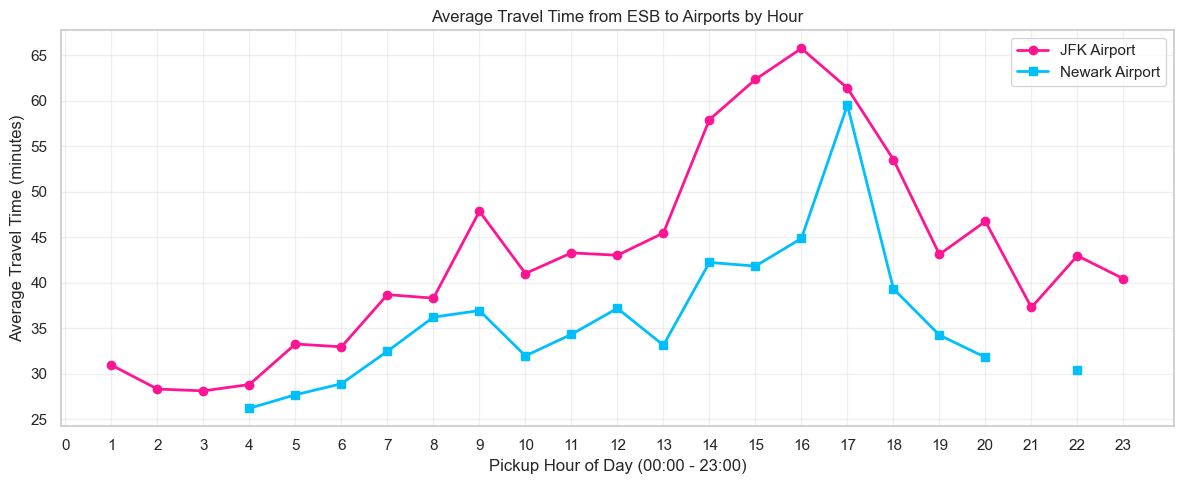
\includegraphics[width=\linewidth]{section5_plots/travel_time_by_hour.png}
    \caption{Average travel time from the ESB area to JFK and Newark by
    pickup hour. Times are in minutes, using the chosen location radii.}
    \label{fig:q5_time_by_hour}
\end{figure}

\textbf{JFK:} The shortest observed averages were in the early morning.
For example, the mean at 04:00 was 28.83 minutes. Travel time generally
increased as the day progressed, especially in the afternoon. It reached
\textbf{65.75 minutes at 16:00}, which was the highest observed hourly
mean for JFK. Between 14:00 and 17:00, the JFK averages were all above
57 minutes.

\textbf{Newark:} The same broad pattern appeared, although Newark was
usually faster. At 04:00, the average was 26.22 minutes. Between 14:00
and 16:00, the averages were approximately 42--45 minutes. The highest
observed Newark average was \textbf{59.50 minutes at 17:00}, but only
four trips contributed to that value, so it is less reliable than an
average based on many journeys.

A possible reason for longer afternoon journeys is heavier road traffic.
Different route lengths and the bridges, tunnels or roads used may also
contribute to the difference between the airports. However, the dataset
does not contain direct traffic measurements or the routes followed.
These are therefore \emph{possible explanations}, not proven causes.

\subsection*{Number of trips and reliability of the hourly averages}

\begin{figure}[H]
    \centering
    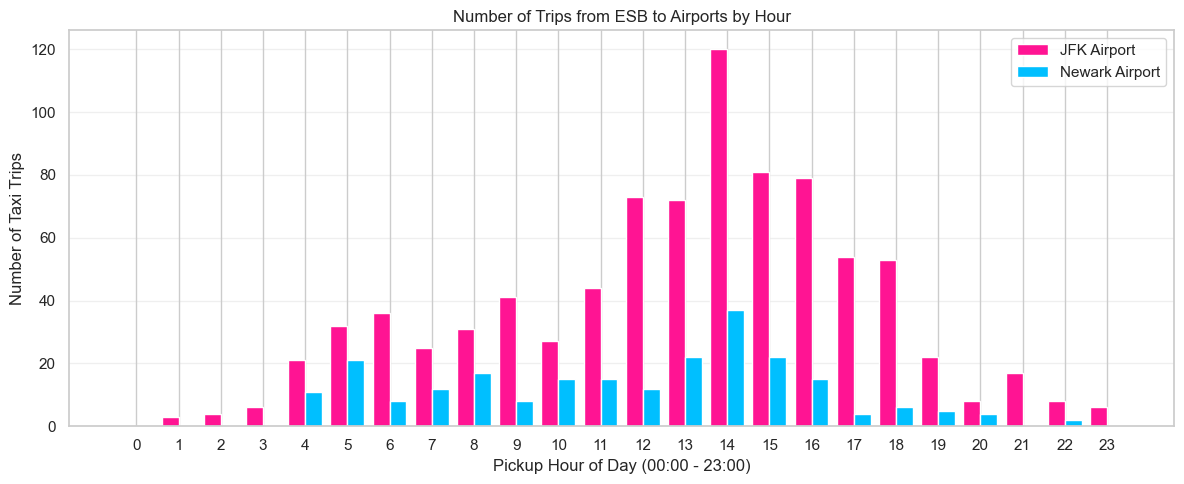
\includegraphics[width=\linewidth]{section5_plots/trips_by_hour.png}
    \caption{Number of ESB-to-airport trips by pickup hour. These are
    the sample sizes behind the hourly averages in
    Figure~\ref{fig:q5_time_by_hour}.}
    \label{fig:q5_counts_by_hour}
\end{figure}

The largest number of trips to both airports occurred at 14:00:
\textbf{120 JFK trips} and \textbf{37 Newark trips}. There were also
\textbf{79 JFK trips at 16:00}, supporting the interpretation that the
high JFK travel-time average at that hour is based on a substantial
number of journeys. By contrast, Newark had only four trips at 17:00,
so its sharp peak of 59.50 minutes should be interpreted cautiously.
Newark also had no matching trips for several late-night hours, so no
hourly average can be estimated for those hours from this sample.

\end{document}
